\documentclass[tikz]{standalone}
\usepackage{pgfplots}
\usepackage{upgreek}


\definecolor{CUHKorange}{RGB}{244,106,18} %F47012
\definecolor{CUHKblue}{RGB}{0,111,190}    %006FBE
% #B2m = #33A02C
% #B1 = #1F78B4
% #B2v = #6A3D9A
% #B1opc=#FF7F00

\definecolor{mygreen}{HTML}{33A02C}
\definecolor{myblue}{HTML}{1F78B4}
\definecolor{mypur}{HTML}{6A3D9A}
\definecolor{myorg}{HTML}{FF7F00}

\begin{document}
\pgfplotsset{
    width=0.90\linewidth,
    height=0.3\linewidth
}
\noindent
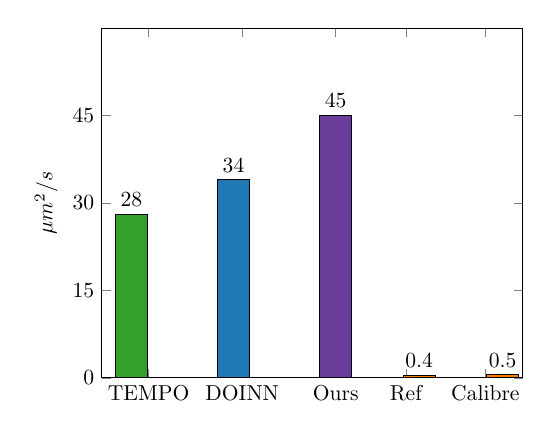
\begin{tikzpicture}[scale=.78]
    \begin{axis}[
        ybar,
        %xlabel={Benchmarks},
        xticklabels={TEMPO, DOINN, Ours, Ref, Calibre},xtick={1, 3, 5, 6.5, 8.2},
        xtick align=inside,
        xticklabel style={rotate=0},
        ylabel={$\mu m^{2} / s$},
        ytick={0, 15, 30, 45},
        ylabel near ticks,
        nodes near coords,
        nodes near coords style={color=black},
        bar width = 15pt,
        xmin=0,
        xmax=9,
        ymin=0,
        ymax=60,
        legend style={at={(0.5,1.25)},
        draw=none,anchor=north,legend columns=-1},
    ]
    % use TeX as calculator:
    \addplot +[ybar, fill=mygreen,  draw=black, area legend] coordinates {(2.2, 28)};
    \addplot +[ybar, fill=myblue,  draw=black, area legend] coordinates {(3.6, 34)};
    \addplot +[ybar, fill=mypur,  draw=black, area legend] coordinates {(5, 45)};
    \addplot +[ybar, fill=myorg,  draw=black, area legend] coordinates {(6, 0.4)};
    \addplot +[ybar, fill=myorg,  draw=black, area legend] coordinates {(7, 0.5)};
    \end{axis}
\end{tikzpicture}
\end{document}
